\documentclass[12pt,a4paper,openright,twoside]{book}
\usepackage[utf8]{inputenc}
\usepackage{disi-thesis}
\usepackage{code-lstlistings}
\usepackage{notes}
\usepackage{shortcuts}
\usepackage{acronym}
\usepackage{listings}
\usepackage{xcolor}

\school{\unibo}
\programme{Corso di Laurea in Ingegneria e Scienze Informatiche}
\title{Integrazione di RAG e LLM nello Sviluppo del Software}
\author{Bollini Simone}
\date{\today}
\subject{Programmazione ad oggetti}
\supervisor{Prof. Viroli Mirko}
\cosupervisor{Dott. Aguzzi Gianluca}
\morecosupervisor{Dott. Farabegoli Nicolas}
\session{IV}
\academicyear{2023-2024}

% Definition of acronyms
\acrodef{RAG}{Retrieval-Augmented Generation}
\acrodef{AI}{Artificial intelligence}
\acrodef{LLM}{Large Language Model}


\mainlinespacing{1.241} % line spacing in mainmatter, comment to default (1)

\begin{document}

\frontmatter \frontispiece

\begin{abstract}	
I \ac{LLM} addestrati per sviluppare il codice sono oggi altamente efficaci e in grado di generare soluzioni utili e funzionanti.
L'addestramento fatto sui modelli è però su fonti e soluzioni generali, questo non da quindi la possibilità al modello di proppore soluzioni su misura per una specifica richiesta utilizzando casistiche già create dal programmatore o dalla propria azienda per casi simili. Da questo nasce l'esigenza di addestrare il modello per personalizzare le soluzioni proposte, contestualizzandole alla propria realtà aziendale e al proprio stile nel programmare.
Il \ac{LLM} non conosce le librerie interne dell'azienda, i pattern di programmazione adottati e quindi le risposte ottenute sono troppo generiche.
Per rispondere a questa esigenza entra in gioco la \ac{RAG} ovvero il processo di ottimizzazione dell'output di un \ac{LLM},
per permettergli di fruire di un ulteriore base di conoscenza personalizza, unica e privata.
L'outup di questa \textbf{matrice di conoscenza} si inserisce e completa la query inviata al LLM, estendendo la base di informazioni sulla quale genererà l'output con la risposta.
Questa tesi approfondisce questi concetti e sperimenta l'integrazione di un \ac{RAG} con un \ac{LLM} con lo scopo di ottenere dal LLM risposte personalizzate
che solo con la conoscenza del LLM anche se estremamente performante e preparato sarebbe stato impossibile ottenere.
\end{abstract}

\begin{dedication}
A Giulia e ai miei figli, il dono più grande.
\newline A tutta la mia famiglia.
\newline Grazie a tutti voi.
\end{dedication}

%----------------------------------------------------------------------------------------
\tableofcontents   
\listoffigures     % (optional) comment if empty
%\lstlistoflistings % (optional) comment if empty
%----------------------------------------------------------------------------------------

\mainmatter

%----------------------------------------------------------------------------------------
\chapter{Introduzione}
\label{chap:introduction}
%----------------------------------------------------------------------------------------

\section{Essere programmatori nel 2025}
Sono disponibili tantissimi (IDE) per lo sviluppo del codice uno di questi è \textbf{Visual Studio Code},
mentre \textbf{Github} può essere lo strumento utilizzato condividere progetti per lavore in maniera collaborativa.
Se richiesta memoria GPU per piccoli progetti accademici è disponibile \textbf{COLAB} che permette di eseguire in remoto codice offrendo anche gratuitamente utilizzo di GPU.
Questi esempi mostrano una panoramica di strumenti vasta, complessa e in rapita evoluzione, con un frequente cambio di software per realizzare un programma.
Un esempio d'utilizzo con gli strumenti sopra elencato potrebbe essere la realizzazione iniziale del progetto in locale utilizzado Visual Studio Code per poi riportare il tutto su GitHub.
In un secondo momento il codice viene ripreso e aperto su Colab dove a sua volta il programma viene modificato ed infine rieseguito il Push sul progetto radice presente su GitHub.
Ora nel 2025, la cosa che accomuna questi strumenti, è l'implemazione al loro interno di funzioni che basate sull'IA, in grado di completare il codice, suggerire correzioni e creare documentazione pertinente.
Un esempio semplice ma che offre già un idea della vastità e della potenza di queste funzioni è l'utility di \textbf{Github Copilot} 'Generate Commit Message with Copilot'
che propone il testo da utilizzare come descrizione di un commit, ho provato a riscontrare quanto fosse contestualizzato e coerente 
con quanto aggiornato e ho ottenuto il seguente risultato:
\begin{figure}[h]
    \centering
    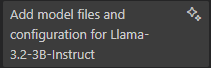
\includegraphics[width=0.5\linewidth]{figures/commit.png}
    \label{fig:Commeit-Autogenerato}
\end{figure}
\newline
Nel mio caso quanto proposto era corretto ed ho quindi eseguito il Commit con la descrizione proposta.
Quanto è riuscito a fare Copilot è strabiliante, in pochi istanti ha analizzato il contesto ritornando come output una risposta semplice ma coerente rispetto a quanto cambiato.
L'uso di questi strumenti sta rendendo il lavoro molto più dinamico e veloce, riducendo le interruzioni nel cercare soluzioni o per trovare le giuste parole per descrivere
quanto fatto.
\begin{figure}[h]
    \centering
    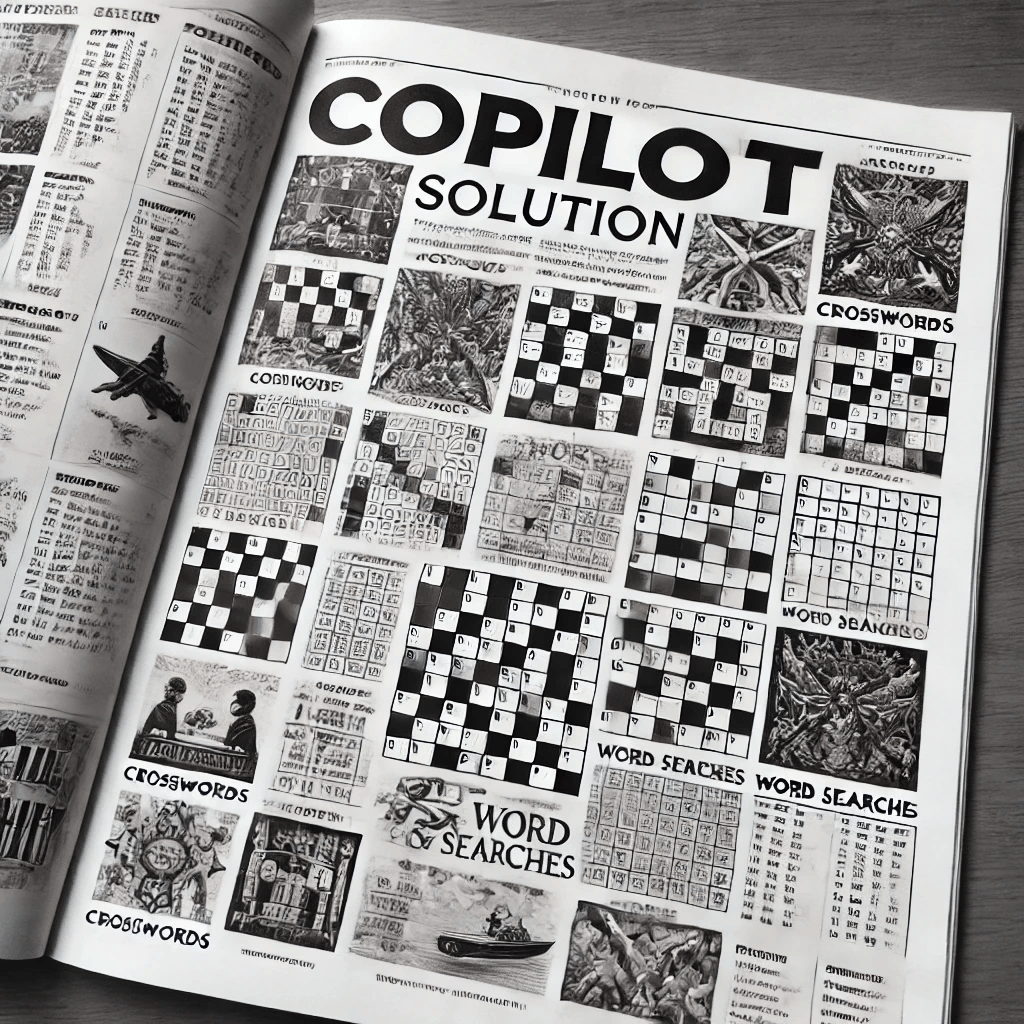
\includegraphics[width=0.5\linewidth]{figures/copilotsolutionSettimanaEnigmistica.png}
    \label{fig:Copilot-Solution}
\end{figure}
\newline
L'intelligenza artificiale sta rivoluzionando il modo in cui il software viene sviluppato, strumenti come Copilot utilizzando tutto il loro potenziale, possono creare la spina dorsale di un progetto
in pochi secondi lasciando al programmatore il compito di verificare e correggere solo in parte il codice proposto. 
In progetti complessi questo non riduce il ruolo del programmatore, anzi lo eleva a compiti di precisione e ad alto valore aggiunto lasciando la stesura di parti del codice semplici e ripetitive al software stesso.
Sapere cosa chiedere e formulare correttamente le domande al LLM è fondamentale, esplicitando nel dettaglio con parole chiave mirate come deve essere realizzato il codice.
Altro compito complesso per il programmatore è non farsi troppo ammaliare dalle soluzioni proposte perché non sempre necessarie per quanto richiesto oppure diverse da quanto già conosciuto
 per realizzare una determinata funzione.
Questo nuovo modo di lavorare per mette di conoscere nuove soluzioni ma comporta test e tempo non sempre disponibile,
il programmatore deve sempre avere il controllo del progetto accettando generazione del codice automatica solo dove consapevole di quanto proposto e del suo impatto anche in casi di revisione e manutenzione futuri.
L'ultimo miglio da percorrere per sfruttare questi strumenti è la personalizzazione delle risposte del LLM, per ottenere risposte coerenti con quanto già realizzato e conosciuto, per fare questo entra in gioco la RAG.
\chapter{Addestrare un LLM per la Generazione del Codice}

L'addestramento di LLM per la generazione di codice di programmazione richiede una serie di passaggi metodici e risorse computazionali significative.
Conoscere questo processo è utile per la successiva integrazione con la RAG.
La procedura si divide nelle selle seguenti fasi:

\section{Raccolta e Preparazione dei Dati}

La qualità e la quantità dei dati per l'addestramento è di primaria importanza per prepare un modello alla generazione di codice in maniera efficace.
È quindi essenziale utilizzare per il training codice sorgente proveniente da molteplici fonti tra cui codice sorgente, file Readme, documentazione tecnica, commenti nel codice,
pagine Wiki, API e discussioni su forum specializzati in programmazione.
In rete è possibile trovare diverso materiale open source tra cui dataset già etichettati. Alcuni dataset hanno un valore altissimo, per tutelare il costo per produrli per certi dataset è previsto il diritto d'autore.
I dati si dividono in due tipologie:
\begin{itemize}
    \item \textbf{Dati Strutturati}: seguono un formato specifico e predefinito.
    \item \textbf{Dati non Strutturati}: non sono organizzati e sono quindi più difficili da interpretare dal modello. 
\end{itemize}
La raccolta di dati va visionata con cura, se non si conosce la provenienza del codice è possibile che contenga bug o codice opsoleto che possono essere trasmessi al modello.
I dati raccolti devono essere quindi puliti e pre-processati per rimuovere errori e informazioni non pertinenti, garantendo così un dataset di alta qualità per l'addestramento.
Sui dataset viene utilizzato un tokenizer specializzato che riconosce costrutti di programmazione come keyword, operatori e strutture sintattiche.

\section{Pre-Addestramento}
Il pre-addestramento di un LLM  da utilizzare per la generazione di codice richiede un approccio specifico.
A differenza del pre-addestramento generico, utilizzando i dataset precedentemente prepareti il modello impara a:
\begin{itemize}
    \item Predire il completamento del codice
    \item Comprendere la struttura sintattica dei linguaggi di programmazione
    \item Riconoscere pattern comuni nel codice
    \item Identificare le relazioni tra diversi blocchi di codice
\end{itemize}
Un esempio pratico di pre-addestramento può essere implementato utilizzando la libreria transformers \cite{huggingface-transformers, codebert}:

\begin{lstlisting}[language=Python]
from transformers import RobertaConfig, RobertaTokenizerFast

# Configurazione del modello per il codice
config = RobertaConfig(
    vocab_size=50000,  # Dimensione del vocabolario
    max_position_embeddings=514,  # Lunghezza massima sequenza
    num_attention_heads=12,  # Teste di attenzione
    num_hidden_layers=6,  # Strati nascosti
    type_vocab_size=1  # Tipo di vocabolario
)

# Tokenizer specializzato per il codice
tokenizer = RobertaTokenizerFast.from_pretrained(
    "microsoft/codebert-base",
    max_length=512,
    truncation=True,
    padding=True
)
\end{lstlisting}

Durante questa fase, il modello sviluppa una comprensione profonda della sintassi e della semantica del codice, che verrà poi raffinata durante il fine-tuning per compiti specifici di generazione del codice.
\section{Fine-Tuning}
Il fine-tuning è la fase in cui il modello viene specializzato per la generazione di codice, documentazione e risposta a quesiti specifici del contesto di programmazione. Durante questa fase, il modello affina le sue capacità attraverso:

\begin{itemize}
    \item \textbf{Dataset Specializzati}: Utilizzo di dataset contenenti:
    \begin{itemize}
        \item Coppie di descrizioni-implementazioni
        \item Documentazione tecnica e commenti
        \item Esempi di bug fixing e refactoring
    \end{itemize}
    
    \item \textbf{Tecniche di Apprendimento}:
    \begin{itemize}
        \item \textbf{Apprendimento Supervisionato}: Training su coppie input-output predefinite
        \item \textbf{Apprendimento per Rinforzo}: Ottimizzazione basata su feedback e metriche di qualità
        \item \textbf{Few-shot Learning}: Adattamento a nuovi contesti con pochi esempi
    \end{itemize}
\end{itemize}

Un esempio pratico di fine-tuning può essere implementato utilizzando la libreria transformers \cite{huggingface-transformers}:

\begin{lstlisting}[language=Python]
from transformers import Trainer, TrainingArguments
from datasets import load_dataset

# Caricamento del dataset per il fine-tuning
dataset = load_dataset("code_search_net", "python")

# Configurazione del training
training_args = TrainingArguments(
    output_dir="./results",
    num_train_epochs=3,
    per_device_train_batch_size=8,
    per_device_eval_batch_size=8,
    warmup_steps=500,
    weight_decay=0.01,
    logging_dir="./logs",
    logging_steps=10,
    evaluation_strategy="epoch"
)

# Inizializzazione del trainer
trainer = Trainer(
    model=model,                # Modello pre-addestrato
    args=training_args,         # Argomenti di training
    train_dataset=dataset["train"],
    eval_dataset=dataset["validation"],
    tokenizer=tokenizer,        # Tokenizer specializzato per il codice
)

# Avvio del fine-tuning
trainer.train()
\end{lstlisting}

Durante il fine-tuning, il modello sviluppa capacità specifiche come:
\begin{itemize}
    \item Generazione di codice a partire da descrizioni in linguaggio naturale
    \item Completamento intelligente del codice basato sul contesto
    \item Creazione di documentazione tecnica
    \item Identificazione e correzione di bug
    \item Refactoring del codice seguendo best practices
\end{itemize}

Il processo di fine-tuning richiede un attento bilanciamento tra:
\begin{itemize}
    \item \textbf{Overfitting}: Evitare che il modello memorizzi i dati di training
    \item \textbf{Generalizzazione}: Mantenere la capacità di adattarsi a nuovi contesti
    \item \textbf{Prestazioni}: Ottimizzare la velocità e la qualità delle risposte
\end{itemize}

\section{Pre-Addestramento vs Fine-Tuning}
È importante comprendere la distinzione tra queste due fasi dell'addestramento:
\subsection{Pre-Addestramento}
Il pre-addestramento è la fase iniziale dove il modello:
\begin{itemize}
    \item Acquisisce una comprensione \textbf{generale} del linguaggio di programmazione
    \item Viene addestrato su \textbf{grandi quantità} di codice sorgente generico
    \item Impara le strutture base e la sintassi del linguaggio
    \item Non è ancora specializzato per compiti specifici
\end{itemize}

\subsection{Fine-Tuning}
Il fine-tuning è invece la fase di specializzazione dove il modello:
\begin{itemize}
    \item Si adatta a un \textbf{dominio specifico} o a compiti particolari
    \item Utilizza dataset più piccoli ma \textbf{mirati}
    \item Affina le conoscenze per generare codice per specifici casi d'uso
\end{itemize}

\textbf{Analogia}: Si può paragonare a:
\begin{itemize}
    \item Pre-addestramento: Imparare la grammatica e il vocabolario di base di una lingua
    \item Fine-tuning: Specializzarsi nel linguaggio tecnico di un settore specifico
\end{itemize}

\section{Architettura del Modello}
Gli LLM utilizzano tipicamente architetture basate su trasformatori, che sono particolarmente efficaci nell'elaborazione di sequenze di dati, come il testo e il codice.
I trasformatori utilizzano meccanismi di auto-attenzione per valutare l'importanza di diversi elementi in una sequenza,
permettendo al modello di comprendere le relazioni tra parole o token.
Questa capacità è fondamentale nella generazione del codice, poiché le dipendenze tra variabili e funzioni possono estendersi su ampie sezioni del codice, richiedendo al modello di considerare un ampio contesto per trovare le risposte corrette.

\section{Valutazione e Ottimizzazione}
Una volta addestrato, il modello deve essere rigorosamente valutato utilizzando metriche specifiche per la generazione di codice, come la correttezza sintattica, la funzionalità e l'efficienza del codice prodotto.
I risultati della valutazione possono essere utilizzati per ulteriori ottimizzazioni, come aggiustamenti dei pesi del modello, modifiche all'architettura o includere dati di addestramento aggiuntivi per affrontare eventuali carenze.

\subsection{Metriche di Valutazione}
\begin{itemize}
    \item \textbf{Correttezza Sintattica}: Verifica che il codice generato sia sintatticamente corretto.
    \item \textbf{Funzionalità}: Verifica che il codice generato realizzi la funzionalità desiderata.
    \item \textbf{Efficienza}: Valuta le prestazioni del codice in termini di tempo di esecuzione e utilizzo delle risorse.
\end{itemize}

\subsection{Tecniche di Ottimizzazione}
\begin{itemize}
    \item \textbf{Aggiustamento dei Pesi}: Modifica dei pesi del modello per migliorare le prestazioni.
    \item \textbf{Modifiche all'Architettura}: Introduzione di nuove componenti o modifiche a quelle esistenti.
    \item \textbf{Integrazione di Dati Aggiuntivi}: Utilizzo di ulteriori dati di addestramento per migliorare le prestazioni.
\end{itemize}

\chapter{RAG}
\section{Introduzione}
Il RAG \textbf{Retrieval-Augmented Generation}, (in italiano \textit{Generazione Aumentata tramite Recupero} )  è un sistema che permette di migliorare l'output di un LLM estendendo la sua conoscenza con nuove informazioni, al di fuori dai suoi dati di addestramento.
Allo scopo di:
\begin{itemize}
    \item ottenere risposte personalizzate provenienti da librerie e codice custom;
    \item migliorare il codice generato rendendolo più specifico al dominio riducendo le allucinazioni;
    \item facilitare l'assistenza da parte del modello nella fase di debugging migliorando la sua comprensione di sistemi complessi;
    \item supportare la creazione di documentazione aggiornata;
    \item permettere all'interno di un Team di migliorare la coerenza del codice scritto da diversi programmatori;
    \item realizzare naturalmente senza forzature, codice più moderno proponendo librerie e standard comuni.
    \item evitare risposte imprecise a causa della confusione terminologica, in cui diverse fonti utilizzano la stessa terminologia per parlare di cose diverse.
\end{itemize}

\section{Funzionamento}

\begin{figure}[h]
    \centering
    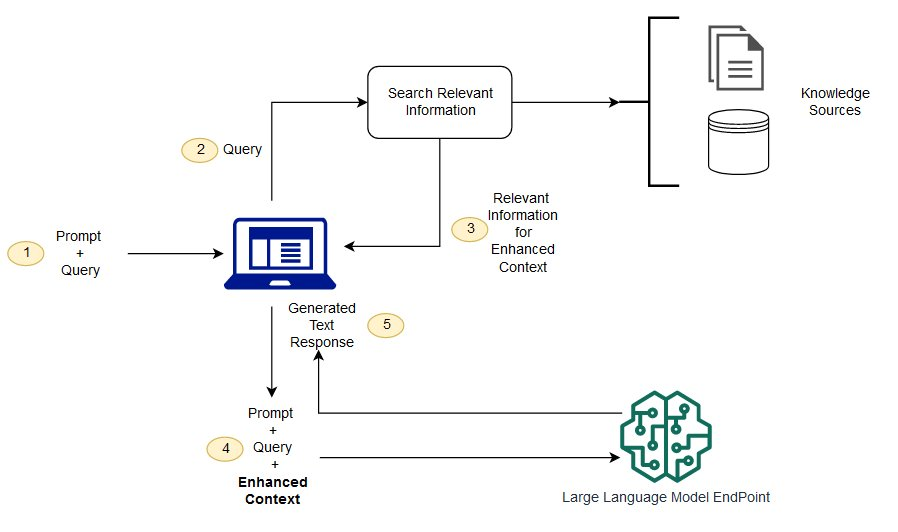
\includegraphics[width=.8\linewidth]{figures/jumpstart-fm-rag.jpg}
    \caption{Flusso di una request ad un LLM integrato con un RAG}
    \label{fig:jumpstart-fm-rag}
\end{figure}
RAG è un sistema che integra il processo di generazione del linguaggio con un meccanismo di recupero delle informazioni. Il funzionamento si articola in diverse fasi, come illustrato in \cref{fig:jumpstart-fm-rag}.

\subsection{Creazione degli Embedding}
Il sistema RAG utilizza dati esterni al training set originale del LLM, provenienti da diverse fonti come:
\begin{itemize}
    \item API e database interni
    \item Archivi documentali
    \item File di testo e codice
\end{itemize}
Questi dati vengono convertiti in rappresentazioni numeriche (embedding) e archiviati in un database vettoriale, creando una knowledge base accessibile dal RAG.

\subsection{Fase 1: Function Calling}
Il sistema RAG inizia con una chiamata di funzione per ricercare nei dati di embedding:
\begin{itemize}
    \item La query dell'utente attiva una chiamata di funzione
    \item Il sistema cerca nei dati di embedding le informazioni pertinenti
    \item Se trovate, queste informazioni vengono aggiunte al prompt
\end{itemize}

\subsection{Fase 2: Recupero delle Informazioni}
Quando l'utente sottopone una query:
\begin{itemize}
    \item La domanda viene convertita in un vettore
    \item Il sistema cerca nel database vettoriale le informazioni più pertinenti
    \item Viene calcolata la rilevanza attraverso calcoli matematici vettoriali
\end{itemize}

\subsection{Fase 3: Aumento del Prompt}
Il sistema RAG arricchisce il prompt dell'utente:
\begin{itemize}
    \item Aggiunge le informazioni recuperate al contesto
    \item Utilizza tecniche di prompt engineering per ottimizzare la comunicazione con il LLM
    \item Fornisce al modello un contesto arricchito per generare risposte più accurate
\end{itemize}

\section{Gestione dell'Aggiornamento dei Dati}
Per mantenere l'efficacia del sistema nel tempo:
\begin{itemize}
    \item Ricalcolo degli embedding per i nuovi dati
    \item Possibilità di aggiornamenti in tempo reale o batch
\end{itemize}

Questo approccio permette di superare le limitazioni dei LLM, fornendo risposte più accurate e contestualizzate grazie all'integrazione di conoscenze esterne aggiornate.

\chapter{Caso Studio: Implementazione di un Sistema RAG per lo Sviluppo del Software}

\section{Obiettivi del Caso Studio}
Questo caso studio si propone di:
\begin{itemize}
    \item Dimostrare l'applicazione pratica dei concetti teorici presentati nei capitoli precedenti
    \item \textbf{Scenario}: Creare un RAG di supporto allo sviluppo software in una software-house
    \item \textbf{Problematica}: Necessità di generare codice coerente con gli standard e le pratiche aziendali
    \item \textbf{Soluzione Proposta}: Sistema RAG integrato con LLM per la generazione di codice contestualizzato
\end{itemize}


\section{Architettura del Sistema}
(da completare)
[Librerie Custom] → [Chunking] → [Embedding] → [Vector DB] → [Retrieval] → [LLM] → [Risposta contestuale]
% \begin{figure}[h]
%     \centering
%     \includegraphics[width=.8\linewidth]{figures/rag-architecture.png}
%     \caption{Architettura del sistema RAG implementato}
%     \label{fig:rag-architecture}
% \end{figure}

\section{Software Utilizzati}
\subsection{Ollama}
Ollama \cite{ollama-docs} è un software che permette di utilizzare in locale LLM, facilitando la creazione, l'addestramento e l'integrazione di modelli di machine learning nelle applicazioni senza dover dipendere da servizi cloud esterni.
\subsection{LLM}
Per rendere più completa la ricerca sono stati utilizzati due modelli di linguaggio per il caso studio:
\subsubsection{Llama 3.2}
Llama 3.2 3B \cite{llama3-2}, un modello di linguaggio open source sviluppato da Meta AI.
Il modello, con 3 miliardi di parametri, è ottimizzato per compiti di dialogo multilingue e si distingue per le sue capacità di recupero e sintesi delle informazioni.
La scelta è ricaduta su questa versione per il suo equilibrio tra prestazioni e requisiti computazionali che permottono il suo utilizzo senza hardware troppo potente.

\subsubsection{qwen2.5-coder:3b}
qwen2.5-coder \cite{qwen-coder} è stato sviluppato da Qwen AI ed è anchesso open source, specializzato nella generazione di codice e documentazione tecnica.
Con 3 miliardi di parametri, il modello è stato addestrato su un ampio dataset di codice sorgente e documentazione tecnica, permettendo di generare codice coerente e ben strutturato. 
La scelta di questo modello è stata dettata, a differenza di llama3.2, dalla sua specializzazione nella programmazione e dalla sua capacità di generare codice di alta qualità.

\subsection{LangChain}
LangChain \cite{langchain} è un framework open source progettato per la gestione di dati strutturati e non strutturati in contesti multilingue. Fornisce strumenti avanzati per la creazione e la gestione di database vettoriali, facilitando l'organizzazione e la ricerca di informazioni in modo efficiente. LangChain è stato scelto per la sua capacità di integrare modelli di linguaggio con fonti di dati esterne.

\subsection{BGE-M3}
BGE-M3 \cite{bge-m3} è un database vettoriale open source per la gestione di dati strutturati e non strutturati multilingue, sviluppato da BigGraph Engine.


\section{Dataset}
Il dataset utilizzato per il caso studio è una classe custom di prova DateUtil.java simile ad una personalizzata utilizzata in qualsisi azienda per gestire il formato delle date.

\section{Implementazione}
\subsection{Creazione dei Chunk}
Per suddividere il file Java in chunk viene utilizzata la libreria \textbf{langchain\_text\_splitters.}
Il seguente codice Python mostra come suddividere il file Java in chunk di dimensione fissa, salvando i risultati in un file JSON.
\begin{lstlisting}[language=Python, caption={Codice Python per la suddivisione del file Java in chunk}, label={lst:chunking}]
    from langchain_text_splitters import RecursiveCharacterTextSplitter
    import json
    
    # Carica il file Java
    with open("my_project/DateUtil.java", "r") as f:
        java_code = f.read()
    
    # Suddividi il codice in chunk
    splitter = RecursiveCharacterTextSplitter(
        chunk_size=512,  # Dimensione di ogni chunk
        chunk_overlap=128,  # Overlap tra chunk
        separators=["\n\n", "\n", " ", ""]  # Separatori per il codice
    )
    
    chunks = splitter.split_text(java_code)
    
    # Salva i chunk in un file JSON
    chunks_data = [
        {
            "id": i + 1,
            "text": chunk,
            "source": "DateUtil.java",  # Nome del file
            "type": "code",             # Tipo di contenuto
            "start_line": 0,            # Linea di inizio (da calcolare)
            "end_line": 0               # Linea di fine (da calcolare)
        }
        for i, chunk in enumerate(chunks)
    ]
    with open("chunks.json", "w", encoding="utf-8") as f:
        json.dump(chunks_data, f, indent=4, ensure_ascii=False)
    \end{lstlisting}


    \subsection{Generazione degli Embedding}
    Il seguente codice Python mostra come generare gli embedding per i chunk e creare un database Chroma:
    
    \begin{lstlisting}[language=Python, caption={Codice Python per la generazione degli embedding e la creazione di un database Chroma}, label={lst:embeddings}]
    import json
    from sentence_transformers import SentenceTransformer
    from langchain_community.vectorstores import Chroma
    
    # 1. Carica i chunk dal file JSON
    with open("chunks.json", "r", encoding="utf-8") as f:
        chunks_data = json.load(f)
    
    # Estrai i testi dei chunk
    chunks = [item["text"] for item in chunks_data]
    
    # 2. Carica il modello BGE-M3 e genera gli embedding
    embedder = SentenceTransformer('BAAI/bge-m3')
    embeddings = embedder.encode(chunks, show_progress_bar=True)
    
    # 3. Crea un database Chroma
    vector_store = Chroma.from_texts(
        texts=chunks,  # Testi dei chunk
        embedding=embedder,  # Modello di embedding
        persist_directory="./chroma_db"  # Cartella per salvare il database
    )
    
    print("Database Chroma creato e salvato in ./chroma_db.")
    \end{lstlisting}

\subsection{Esecuzione di una Query sul Database Chroma}
Una volta creato il database Chroma, è possibile eseguire ricerche semantiche sui chunk memorizzati:


\begin{lstlisting}[language=Python, caption={Codice Python per l'esecuzione di una query sul database Chroma}, label={lst:query}]
    # Query di esempio
    query = "Come formattare una data in Java?"
    docs = vector_store.similarity_search(query, k=3)  # k = numero di risultati
    for i, doc in enumerate(docs):
        print(f"Risultato {i+1}:")
        print(doc.page_content)  # Contenuto del chunk
        print("-" * 40)
\end{lstlisting}

\subsection{Creazione Rag}

\subsection{AI Agent}
E' un componente che può chiamare delle funzioni (function calling) nel mio caso search
il LLM capisce se deve chiamare o meno il RAG.
\subsubsection{function calling}
Il function calling è un meccanismo che permette di chiamare delle funzioni definite in un file esterno, in questo caso il RAG.


\chapter{Conclusioni}

\section{Risultati Ottenuti}
%In questa tesi ho esplorato l'integrazione di RAG e LLM nello sviluppo del software, dimostrando come questi strumenti possano migliorare significativamente il processo di sviluppo. I risultati principali includono:
%\begin{itemize}
%    \item Implementazione di un sistema RAG per la generazione di codice contestualizzato
 %   \item Analisi delle prestazioni e dell'efficacia del sistema
 %   \item Identificazione di potenziali aree di miglioramento
%\end{itemize}

\section{Impatto sullo Sviluppo Software}
L'integrazione di strumenti basati su AI nel processo di sviluppo software sta rivoluzionando il settore. Durante il periodo di sviluppo di questa tesi (Ottobre 2024 - Gennaio 2025), abbiamo osservato:
\begin{itemize}
    \item Rapida evoluzione degli strumenti di AI per lo sviluppo software
    \item Crescente disponibilità di soluzioni open source
    \item Miglioramento continuo nelle capacità di generazione e comprensione del codice
\end{itemize}

\section{Sfide e Prospettive Future}
%Nonostante i progressi significativi, rimangono diverse sfide da affrontare:
%\begin{itemize}
%    \item Bilanciamento tra automazione e controllo umano
%    \item Gestione delle implicazioni etiche
%    \item Necessità di mantenere competenze tecniche fondamentali
%\end{itemize}


%\lstinputlisting[float,language=Java,label={lst:random-code}]{listings/HelloWorld.java}


%----------------------------------------------------------------------------------------
% BIBLIOGRAPHY
%----------------------------------------------------------------------------------------

\backmatter

\nocite{*} % Remove this as soon as you have the first citation

\bibliographystyle{alpha}
\bibliography{bibliography}

\end{document}
